%%%%%%%%%%%%%%%%%%%%%%%%%%%%%%%%%%%%%%%%%%%%%%%%%%%%%%
% INTRODUCTION
%%%%%%%%%%%%%%%%%%%%%%%%%%%%%%%%%%%%%%%%%%%%%%%%%%%%%%

\chapter[From biophysics to computer science]{From biophysics \\ to computer science}

In 1981, Hubel and Wiesel were awarded the Nobel Prize of Medicine for their discovery of visual perception \cite{NP1981}.
They built and tested a model that describes the path of a message from eye to brain.
Simply put, the message is passed on from neuron to neuron (\cref{fig:synapse}), with each neuron compiling the full message from message components.
Lastly, the message is stored into the brain.

\begin{figure}
    \centering
    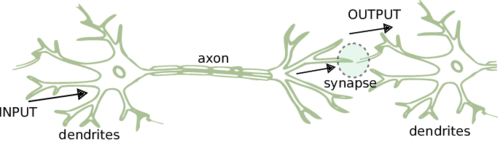
\includegraphics[width=\linewidth]{ANN/images/neural-network.png}
    \caption[Two neurons exchanging information]{
        Information is passed from one neuron to another.
        The message enters the dendrites, passes through the axon, and propagates through the synaptic terminal to another neuron.
        Adapted from \fullcite{Gerstner2002} (Ref.~\cite{Gerstner2002}).
    }
    \label{fig:synapse}
\end{figure}

Inspired by this biological process, artificial neural networks have been developed.
Later, \textcite{Fukushima1980} mimicked this neural network for two dimensional information, using convolution operations.
The approach of \citeauthor{Fukushima1980} was inefficient.
It could not learn to identify reoccurring features.
To enable learning, \textcite{Rumelhart1986} developed backpropagation: an algorithm to learn importances at feature level.
\textcite{LeCun1990} was one of the first to use backpropagation in a visual setting.
They combined convolutions and backpropagation into a convolutional neural network to recognize handwritten digits.

%%%%%%%%%%%%%%%%%%%%%%%%%%%%%%%%%%%%%%%%%%%%%%%%%%%%%%
% BUILDING BLOCKS
%%%%%%%%%%%%%%%%%%%%%%%%%%%%%%%%%%%%%%%%%%%%%%%%%%%%%%

\chapter[CNN building blocks]{The building blocks of convolutional neural networks}

\section{Artificial neural network}
Neural network

\section{Convolutional layers}
To distinguish a neural network from a convolutional neural network (CNN), at least one layer must be a convolution.
A convolution is an operation where a kernel with width $w$ and height $h$ is moved along an input to generate an output.
The output, or output feature map, in two dimensions, is
\begin{equation}
    \mathbf{o}_{i,j} = \mathbf{b}_{i,j} + \sum_{c=0}^{C-1}(\mathbf{x_c} \circledast \mathbf{u}_c)_{i,j}
    = \mathbf{b}_{i,j} + \sum_{c=0}^{C-1}\sum_{n=0}^{w-1}\sum_{m=0}^{h-1}\mathbf{x}_{c,n+i,m+j}\mathbf{u}_{c,n,m},
\end{equation}
where $\mathbf{x}$ is the input possibly containing $C$ multiple channels.
The bias $\mathbf{b}$ and weights $\mathbf{u}$ are learnable parameters.

Convolutions can be modified in a few ways that are important for deep learning.
The first modification is padding, and specifies the size of an added frame around the input.
The frame can have any value, but generally, it is filled with zeros.
A second modification is stride, which specifies the step size with which the kernel moves across the input.

A two-dimensional numerical convolution operation with padding and strides is visualized in \cref{fig:numerical_padding_strides}.
The kernel with size $k=3$ moves across the input of size $i=5$ with stride $s = 2$ in both directions.

Convolutions have the useful property that they are equivariant to translations.
A function $f$ is equivariant to function $g$ if
\begin{equation}
    f \circ g = g \circ f.
\end{equation}
The equivariance of convolutions and translations implies that learned weights and biases belonging to a convolution can be reused for identifying similar features anywhere in inputs.
Moreover, any operator that is not equivariant with convolutions may be used as a way to augment data, as the kernel perceives it is being different.
Examples of such operators are scaling, rotating, and flipping.\marginnote{Move this to its own theory section about data augmentation?}

\begin{figure*}%[p]
    \centering
    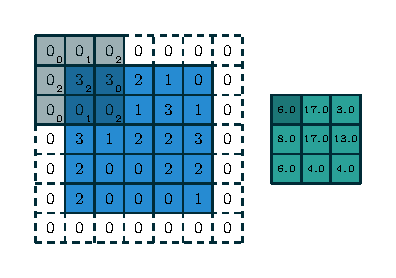
\includegraphics[width=0.32\linewidth]{ANN/images/numerical_padding_strides_00.pdf}
    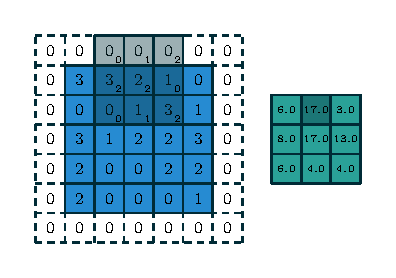
\includegraphics[width=0.32\linewidth]{ANN/images/numerical_padding_strides_01.pdf}
    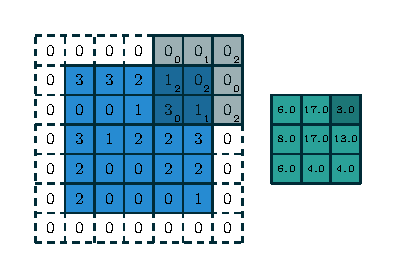
\includegraphics[width=0.32\linewidth]{ANN/images/numerical_padding_strides_02.pdf}
    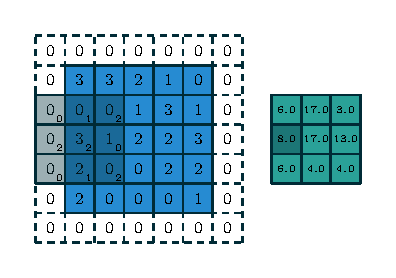
\includegraphics[width=0.32\linewidth]{ANN/images/numerical_padding_strides_03.pdf}
    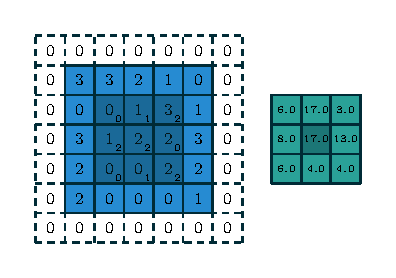
\includegraphics[width=0.32\linewidth]{ANN/images/numerical_padding_strides_04.pdf}
    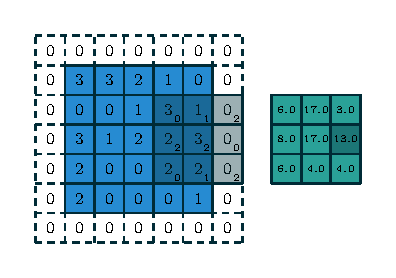
\includegraphics[width=0.32\linewidth]{ANN/images/numerical_padding_strides_05.pdf}
    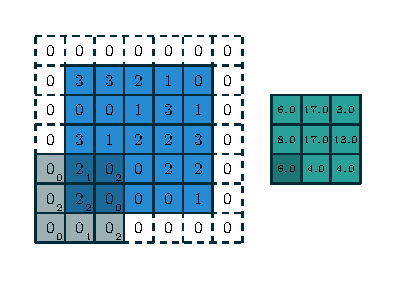
\includegraphics[width=0.32\linewidth]{ANN/images/numerical_padding_strides_06.pdf}
    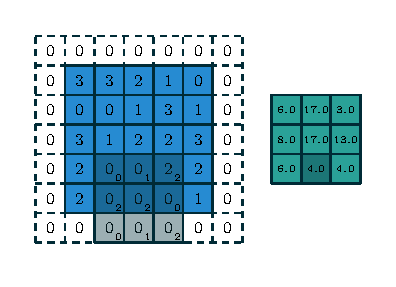
\includegraphics[width=0.32\linewidth]{ANN/images/numerical_padding_strides_07.pdf}
    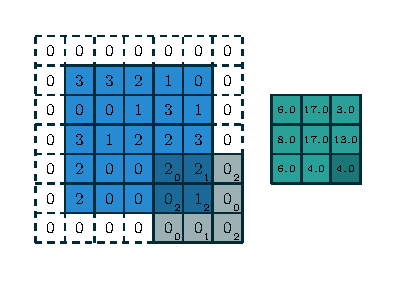
\includegraphics[width=0.32\linewidth]{ANN/images/numerical_padding_strides_08.pdf}
    \caption{Computing the output values
        of a discrete convolution for two dimension, $i_1 = i_2 = 5$, $k_1 = k_2 = 3$,
        $s_1 = s_2 = 2$, and $p_1 = p_2 = 1$.
        Reproduced from \fullcite{Dumoulin2016} (Ref.~\cite{Dumoulin2016}).
    }
    \label{fig:numerical_padding_strides}
\end{figure*}

% \begin{figure*}[p]
%     \centering
%     \includegraphics[width=0.24\textwidth]{ANN/images/arbitrary_padding_no_strides_00.pdf}
%     \includegraphics[width=0.24\textwidth]{ANN/images/arbitrary_padding_no_strides_01.pdf}
%     \includegraphics[width=0.24\textwidth]{ANN/images/arbitrary_padding_no_strides_02.pdf}
%     \includegraphics[width=0.24\textwidth]{ANN/images/arbitrary_padding_no_strides_03.pdf}
%     \caption[Convolution]{
%         Convolving a $4 \times 4$ kernel over a $5 \times 5$ input
%         padded with a $2 \times 2$ border of zeros using unit strides (i.e.,
%         $i = 5$, $k = 4$, $s = 1$ and $p = 2$).
%         Reproduced from \fullcite{Dumoulin2016} (Ref.~\cite{Dumoulin2016}).
%     }
%     \label{fig:arbitrary_padding_no_strides}
% \end{figure*}

\section{Pooling}\label{sec:pooling}
Pooling is a form of nonlinear downsampling.
To achieve this, typically, a convolution kernel is moved over the input with a stride as big as the kernel itself.
This ensures that the downsampling considers measures of input sub-regions.

Pooling is equivariant to any permutation under the kernel.
This results in invariance to local translations.
In deep learning, pooling is therefore used to quantify the presence of a pattern, as opposed to finding its position.

\subsection{Max pooling}\label{subsec:maxpool}
The most common form of pooling is max pooling (ref).
The kernel finds the maximum value in sub-regions and maps these maximum values per sub-region to a new image.
The output
\begin{equation}
    \mathbf{o}_{c, i, j} = \max_{n < h, m < w}\mathbf{x}_{c, si+n, rj+m},
\end{equation}
where $rw$ and $sh$ are the width and height of the input.

\subsection{Average pooling}\label{subsec:avgpool}
Another popular form of pooling is the average pooling, which finds the mean value in sub-regions.
The output
\begin{equation}
    \mathbf{o}_{c, i, j} = \frac{1}{wh}\sum_{n=0}^{w-1}\sum_{m=0}^{h-1}\mathbf{x}_{c,si+n,rj+m}.
\end{equation}

\section{Activation functions}\label{sec:activations}

\begin{enumerate}
    \item heaviside
    \item logistic curves
    \item vanishing gradient problem -> relu
\end{enumerate}

\subsection{Vanishing gradient problem}
Over the years, neural networks have become deeper, \ie more layers are being added.

Sigmoids (and other saturating curves like hyperbolical tangent) have.

\subsection{Rectified linear unit}\label{subsec:relu}
To overcome the vanishing gradient problem, non-saturating activation functions can be used.
One such function is the rectified linear unit (ReLU).
It is defined as
\begin{equation}
    f(x) = x^+ = \max(0, x),
\end{equation}
such that only the positive arguments keep their value.


% --------------------------------------------------
% Loss functions
% --------------------------------------------------

\section{Loss functions}
Backpropagation needs a loss to learn in which direction to update weights.
There is a variety of loss functions available (ref review).

\subsection{Mean absolute error}
One of the most straightforward techniques of calculating the loss is the mean absolute error (MAE).
It measures the average difference between every prediction and target, like
\begin{equation}
    \mathrm{MAE} = \frac{1}{n} \sum_{i=1}^{n} |y_i - y'_i|,
\end{equation}
where $n$ is the number of targets per sample, $y$ the prediction and $y'$ the target.

The MAE loss is forgiving, i.\ e.\ outliers are weighted as much as predictions close to the target.
In training a neural network, focusing on outliers is assumed to be beneficial, as those are the cases that the model has difficulty with (ref).

\subsection{Mean square error}
To overcome the forgiving nature of the MAE loss, the mean square error (MSE) can be used.
It measures the average squared difference between every prediction and target, like
\begin{equation}
    \mathrm{MSE} = \frac{1}{n} \sum_{i=1}^n (y_i - y'_i)^2.
\end{equation}

\subsection{Focal MSE}
To give even more focus on the hard targets, giving them more importance than easy targets can be done through the focal MSE loss (FL)~\cite{Lu2022}.
To give less importance to the easier targets, FL follows
\begin{equation}
    FL = \left(\frac{2}{1 + e^{-\beta |y - y'|}} - 1 \right)^\gamma (y_i - y'_i)^2,
\end{equation}
where increasing $\gamma$ increases the number of targets regarded as easy and $\beta$ regulates the speed with which the first part of the curve increases (make fig).

%%%%%%%%%%%%%%%%%%%%%%%%%%%%%%%%%%%%%%%%%%%%%%%%%%%%%%
% TRAINING A NEURAL NETWORK
%%%%%%%%%%%%%%%%%%%%%%%%%%%%%%%%%%%%%%%%%%%%%%%%%%%%%%

\chapter{Training a neural network}

% --------------------------------------------------
% Hyperparameter optimization
% --------------------------------------------------

\section{Hyperparameter optimization}\label{sec:hparam}

A machine learning model uses training data to learn parameters to map input to output data best.
However, there are parameters that cannot be learned, but greatly influence the training outcome.
These parameters are hyperparameters.
Examples of hyperparameters are the batch size, learning rate, learning rate scheduler and its parameters, optimizer algorithm, etc.
These parameters span a configuration space $\mathcal{C}$.
Parameters can be categoral (type of optimizer, learning rate scheduler, etc.) or integers (batch size, number of iterations, etc.), or continuous decimals (learning rate, weight decay, etc.).
Ideally, parameters are sampled exhaustively.
This way, the best possible set of parameters can be found.
However, this can be computationally expensive.
Moreover, when using a continuous variable, it is no long possible to exhaustively sample parameters.
To engage this problem, various algorithms have been developed to sample hyperparameters from the high-dimensional distribution.

\subsection{Grid search and random search}
The most straightforward technique of finding the best set of hyperparameters is grid search.
With grid search, parameters are sampled exhaustively using equidistant spacing in each dimension.

A drawback of grid search is that optima can reside outside the hyperparameter set that grid search produces.
Random search \cite{Bergstra2012} aims to find optima in the gaps using random search.
With the same number of trials, random search has a higher probability for trials to find the global optimum.
This is because trials explore the whole distribution as opposed to just a few points in individual dimensions.
\Cref{fig:gridrandsearch} shows the differences between grid search and random search and advocates the use of the latter.

\begin{figure}
    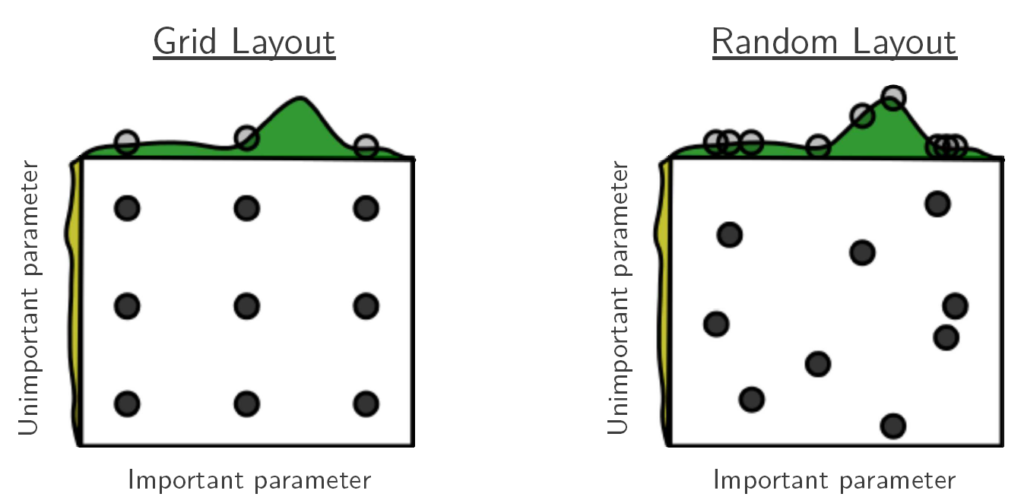
\includegraphics[width=\linewidth]{images/gridrandsearch.png}
    \caption[Grid and random search]{
        Grid and random search of nine trials for optimizing a function $f(x, y) = g(x) + h(y) \approx g(x)$ with low effective dimensionality.
        Above each square $g(x)$ is shown in green, and left of each square $h(y)$ is shown in yellow.
        Reproduced from \fullcite{Bergstra2012} (Ref.~\cite{Bergstra2012}).
    }
    \label{fig:gridrandsearch}
\end{figure}

\subsection{Tree Parzen estimator}
Still, random search requires trials in regions that are unpromising.
This is inefficient.
A tree-structured Parzen estimator (TPE)~\cite{Bergstra2011} approach aims to model the probability of a hyperparameter, given a loss value.
That probability consists of two distributions, describing the good and bad values:
\begin{equation}
    p(c|L) =
    \begin{cases}
        p(c|L > L^*) = p(c|\mathrm{bad}) \\
        p(c|L \leq L^*) = p(c|\mathrm{good}),
    \end{cases}
\end{equation}
where $c$ is drawn from $\mathcal{C}$ and $L$ is the loss.
$L^*$ a loss above which losses are considered bad.
TPE chooses $L^*$ to be a fraction of observed $L$ values, such that $p(\mathrm{good}) = \gamma$.
A promising candidate has low probability under $p(c|\mathrm{bad})$ and high probability under $p(c|\mathrm{good})$.
Therefore, $c$ is promising if
\begin{equation}
    \mathrm{promisingness}(c) \propto p(c|\mathrm{good}) / p(c|\mathrm{bad})
\end{equation}
is high.
Ref.~\cite{Bergstra2011} shows that this ratio is proportional to the expected improvement~\cite{Jones2001}.
The configuration responsible for the maximum of $\mathrm{promisingness}(c)$ is used as the next trial.
Results of that trial are now categorized as good or bad, and the iterative process continues.\marginnote{add multivariate note \cite{Falkner2018}}

\subsection{Successive Halving and Hyperband}
Although $\mathcal{C}$ can be sampled more efficiently with TPE, trials still use the full computational budget, even if it is apparent that the trial is unpromising early on.
Early terminating (or pruning) these underperforming trials speeds up hyperparameter optimization.
Pruning trials can be done using Successive Halving (SH)~\cite{Jamieson2016}.
Given a computational budget $B$, \eg number of epochs, the number of trials $T$, and the halving rate $\gamma$, SH performs $\log_\gamma(T)$ rounds.
The budget is distributed uniformly over the trials.
Every round, $\qty{100}{\percent} \times 1/\gamma$ of the trials are discarded based on their performance.
Surviving trials are allowed twice the budget and are again discarded when they have used up their budget.
This iterative process continues until one trial remains.

When using SH, two variables need to be considered, and possible manually tuned.
The more available budget, pruning decisions are made more confident.
Higher halving rates lead to more and more aggressive pruning with the risk of pruning good candidates early.

There is a trade-off between $T$ and $B$.
Suppose $T$ is large, then each trial gets a small amount of budget, but many configurations are explored.
Conversely, if $T$ is small, then each trial gets much budget, at the cost of exploring the number of configurations.
This $T/B$ trade-off is addressed by Hyperband (HB)~\cite{Li2016} by performing a grid search over feasible values of $T$.
HB invokes SH multiple times.
Every invocation of SH is called a bracket.
In the end, HB returns the best configuration possible just like SH, but diminishing the dependence on manually choosing a good $T$.

\section{Training}\label{Training}
At the start of training, a neural network has its weights and biases initialized.
Most probably, the model is not capable of mapping input to output in a robust manner.
To achieve this, repeatedly using backpropagation to update the model parameters aims to shape the model in the direction of minimizing the loss between target and model output.
The neural network is presented with the input data in batches.
Every batch, the model is updated with the backpropagation algorithm.
One cycle of using all the batches is called an epoch.
A training consists of multiple epochs.

For every $\mathcal{B}$th batch, a loss $\mathcal{L}_\mathcal{B}$ can be defined that is used by backpropagation to penalize the model performance.
Taking the average of all batch losses is the epoch loss,
\begin{equation}
    \mathcal{L}_\mathrm{epoch} = \frac{1}{N_\mathcal{B}}\sum_{i=0}^{N_\mathcal{B}}\mathcal{L}_\mathcal{B},
\end{equation}
Tracking $\mathcal{L}_\mathrm{epoch}$ shows how quickly the model is learning.

To see if the model generalizes, it is standard practice to have a hold-out set, that the model does not learn from, but only uses to calculate the validation loss.
Ideally, this validation loss follows a similar trajectory as the training loss.
If the validation loss diverges upwards from the training loss, the model is overfitting.
It fails to generalize to unseen, but similar data.
To remedy this, there are multiple possible solutions.
Solutions include dropout, batch normalization, or more complex models (\ie deeper or wider networks).

\subsection{Dropout}\label{sec:dropout}
Overfitting can be reduced by applying methods of regularization.
One regularization method is dropout.
It prevents neurons from co-adapting, which would otherwise reduce the chance of the model to perform well on external validation sets \cite{Srivastava2014}.
With dropout, individual neurons are activated with probability $p$, effectively dropping neurons randomly.

\subsection{Batch normalization}\label{sec:bn}
Batch normalization (BN)~\cite{Ioffe2015} is a technique to shift and scale batches akin to standardization.
It can be implemented as a layer in any neural network.
Per minibatch and per dimension, the mean and standard deviation of the input are calculated.
Then, the input is standardized with
\begin{equation}
    \hat{x}_i = \frac{x_i - \mu_\mathcal{B}}{\sqrt{\sigma_\mathcal{B}^2 + \epsilon}},
\end{equation}
where $\mu_\mathcal{B}$ and $\sigma_\mathcal{B}$ are the mean and unbiased standard deviation of the batch, and $\epsilon$ is a small number for numerical stability when the variance is small.
The standardized input is then mapped through
\begin{equation}
    y_i = \gamma \hat{x}_i + \beta,
\end{equation}
where $\gamma$ and $\beta$ are learnable parameters learned in a sub-network.

BN has been shown to have a regularizing effect (ref), although combining it with dropout is disputed.
More often than not, using both BN and dropout leads to worse results on the test set.

\subsection{Model ensembling}\label{subsec:model_ensembling}
A benefit of having a cyclic learning rate is generating multiple models across cycles.
The effectiveness of ensembling models from multiple cycles, Snapshot Ensembling, is first described by \textcite{Huang2017}.
During model training, a model can be checkpointed at the best performing epoch for every cycle, see \.
The checkpointed models can be ensembled by choosing the last $m$\marginnote{how many models chosen and how many models checkpointed then?!} out of $n$ models and averaging the output, as
\begin{equation}
    \mathrm{output} = \frac{1}{M} \sum_{i=0}^{m-1} \mathrm{model}_{n-i}(\mathrm{input}).
\end{equation}
\begin{figure}
    \centering
    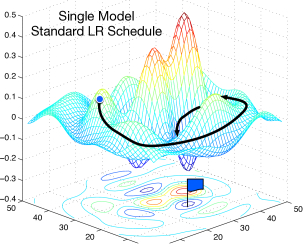
\includegraphics[width=0.48\linewidth]{ANN/images/ensembling_huang_left.png}
    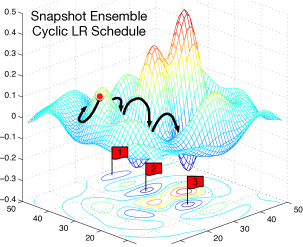
\includegraphics[width=0.48\linewidth]{ANN/images/ensembling_huang_right.png}
    \caption[Snapshot ensembling]{
        Left: Illustration of model optimization The model converges to a local minimum.
        Right: Illustration of Snapshot Ensembling.
        The learning rate is cyclic and annealing, allowing to converge to and escaping from local minima.
        Snapshots are taken at every minimum which can be used for ensembling for inference.
        Reproduced from \fullcite{Huang2017} (Ref.~\cite{Huang2017}).
    }
\end{figure}


% --------------------------------------------------
% Image quality
% --------------------------------------------------

\section{Image quality}\label{subsec:imq}
A convolutional neurel network receives a stream of input images with varying quality.
For example, microscopy images from deep inside tissue are presumably noisier and/or less bright than images taken near the surface.
Neural networks have trouble learning from bad images, as they lack structures that trigger neurons to output predictions close to targets.
Excluding noisy images might increase performance \cite{Blokker2022}.
\textcite{Koho2016} suggest some measures to quantify image quality.
Here, the entropy and kurtosis are discussed.

\subsection{Shannon entropy}
The quality of an image may be described by the amount of information that is contained within it.
The information can be quantified by how surprising it is to contain specific content.
For instance, knowledge that a rare event will occur has high informational value, while knowledge that a probable event will happen has low informational value.
Given a random variable $X$, the information, or entropy, is defined as
\begin{equation}\label{eq:entropy}
    H = \mathbb{E}[-\log p(X)] = -\sum p(x) \log p(x),
\end{equation}
where $\mathbb{E}[\ldots]$ is the expectation operator, and $p(x)$ is the probability of $x$ occurring.
The logarithm satisfies the boundary condition that an event is not surprising if its probability of occurring is one.

For images, \cref{eq:entropy} can be rewritten as
\begin{equation}
    H_I = -\sum_{i}^n P_i \log_2 P_i,
\end{equation}
where $P_i$ is the normalized image histogram at bin index $i$ \cite{Koho2016}.
The base of the logarithm is chosen to be two, such that the entropy is in units of bits.

For images having many different intensities, the entropy is high, because of the knowledge that pixel intensities having lower probability.
The intuition for images with high entropy tending to carry more information is the same as taking images with longer exposure times:
the number of pixels with a certain intensity will increase.
This may be most apparent in dark regions, which would benefit from more illumination.

\subsection{Kurtosis}
Another measure for image quality is kurtosis of the power spectrum.
Kurtosis measures the outliers of a distribution and is given by
\begin{equation}
    \kappa = \frac{\mu_4}{\sigma^4},
\end{equation}
where $\sigma$ is the standard deviation and $\mu_4$ is the fourth moment about the mean.
The $n$th moment about the mean is defined as
\begin{equation}
    \mu_n = \mathbb{E}[(X-\mathbb{E}[X])^n] = \int_{-\infty}^\infty (x-\mu)^n p(x)\,\mathrm{d}x.
\end{equation}
Distributions having a kurtosis of zero are mesokurtic, meaning they resemble a normal distribution.
Posivite kurtosis means that the distribution is leptokurtic.
A leptokurtic distribution has tails with more weight compared to the normal distribution, such as the Poisson or Laplace distribution.
Negative kurtosis means that the distribution is platykurtic.
Platykurtic distributions have thinner tails, such as the Bernoulli distribution.

Kurtosis can be calculated on the upper part of the power spectrum of an image \cite{Koho2016,Blokker2022}.
If the upper part of the power spectrum is very leptokurtic compared to other images in the dataset, it may indicate that the image is an outlier and is significantly different from the mean.
